\chapter{Soortvorming en macro-evolutie}\label{ch:b2:speciation}

Op een klein eiland van de Galápagos kwamen in 1982 enkele grondvinken met
grote snavels van een naburig eiland aan, en ze bleven. Twintig jaar lang
concurreerden ze met de middelste grondvink die er al woonde om de grote zaden
waar beide de voorkeur aan gaven; toen sloeg de droogte toe, raakten de grote
zaden op, en verhongerden de bewoners met de grootste snavels --- die het
rechtstreeks met de nieuwkomers concurreerden. Binnen één generatie waren de
snavels van de bewoners meetbaar gekrompen, weg van die van de indringers.
Twee soorten die elkaar hadden ontmoet, werden uit elkaar gedreven. Dit
hoofdstuk gaat over het ontstaan van soorten: wat een soort is en wat haar
gescheiden houdt, hoe één populatie er twee wordt, de concurrentie die
populaties uit elkaar drijft wanneer ze elkaar ontmoeten, en het lange zicht
van het fossielenbestand, waar hetzelfde proces, meer dan honderd miljoen keer
herhaald, de stamboom van het leven oplevert.

\section{Wat een soort is}

\begin{definition}[Soort]\label{def:b2:speciation:species}
\index{soortbegrip}\index{biologisch soortbegrip}\index{reproductieve isolatie}
Volgens het \emph{biologische soortbegrip} is een soort een groep populaties
waarvan de leden onderling kunnen voortplanten en vruchtbare nakomelingen
voortbrengen, en die \emph{reproductief geïsoleerd} zijn van andere zulke
groepen: wat een soort verenigt, is \omterm{prop:b2:population-genetics:migration}{genenstroom}, en wat soorten scheidt, is de
afwezigheid ervan. Het begrip werkt voor de seksuele organismen van één tijd en
plaats, en dat is het meeste wat een bioloog tegenkomt; het faalt voor
ongeslachtelijke lijnen (die op gelijkenis worden benoemd), voor fossielen
(die niet te kruisen zijn), en voor de vele gevallen waarin de grens lek is ---
eiken en wilgen die over soortgrenzen heen hybridiseren, eenden waarvan de
soorten in gevangenschap kruisen, ringsoorten waarin naburige populaties
helemaal rond een barrière met elkaar kruisen tot de uiteinden elkaar
ontmoeten en dat niet doen. Andere begrippen vullen de gaten: de
\emph{morfologische} soort (een cluster van gelijke vormen), de
\emph{fylogenetische} (de kleinste herkenbare lijn), de \emph{ecologische}
(een lijn met een eigen niche). Geen ervan is fout; elk meet iets echts, en
soortvorming is het proces waardoor ze tot overeenstemming komen.
\end{definition}

\begin{proposition}[Isolatiemechanismen]\label{prop:b2:speciation:isolation}
\index{isolatiemechanisme}\index{prezygotische isolatie}\index{postzygotische isolatie}\index{regel van Haldane}
\omterm{prop:b2:population-genetics:migration}{Genenstroom} tussen twee populaties wordt gestopt door barrières die vóór of na
de bevruchting werken. \emph{Prezygotisch}: de populaties leven in
verschillende habitats of planten zich in verschillende seizoenen voort
(temporele isolatie: twee kikkers die in verschillende maanden roepen); ze
herkennen elkaars balts niet (gedragsisolatie: de zang van krekels, de
lichtcodes van vuurvliegjes, de dansen van eenden); hun geslachtsorganen of
\omterm{def:b2:angiosperm-reproduction:flower}{bloemen} passen niet (mechanische isolatie); hun gameten versmelten niet
(gametische isolatie: de zaadcelbindende eiwitten van zee-egels, de
$S$-allelen van \cref{ch:b2:angiosperm-reproduction}).
\emph{Postzygotisch}: de hybride sterft als embryo, of leeft maar is
steriel (de muilezel; de hybriden van twee \emph{Drosophila}-soorten), of
is vruchtbaar maar haar eigen nakomelingen zijn dat niet (hybride afbraak).
\emph{\omterm{prop:b2:speciation:isolation}{Regel van Haldane}}: wanneer bij een hybride maar één geslacht steriel
of niet levensvatbaar is, is dat het geslacht met twee verschillende
\omterm{prop:b2:meiosis-heredity:sexlinked}{geslachtschromosomen} --- het mannetje bij zoogdieren en vliegen, het vrouwtje
bij vogels en vlinders --- omdat recessieve onverenigbaarheden op het
X-chromosoom daarin zichtbaar worden. Prezygotische barrières zijn goedkoper,
omdat er geen gameten verspild worden, en selectie bouwt ze op waar de
postzygotische al bestaan.
\end{proposition}

\begin{theorem}[Waarom hybriden falen: het model met twee loci]\label{thm:b2:speciation:dm}
\index{Dobzhansky--Muller-incompatibiliteit}
Twee populaties beginnen met \omterm{def:b2:meiosis-heredity:vocabulary}{genotype} $aabb$. In de ene wordt $a$ vervangen
door $A$; in de andere $b$ door $B$; elke substitutie is neutraal of
gunstig in haar eigen genetische achtergrond, zodat geen van beide populaties
ooit door een minder fitte toestand gaat. Maar $A$ en $B$ zijn nooit samen
getest, en als de combinatie onverenigbaar is --- als het eiwit dat $A$ maakt
niet kan samenwerken met het eiwit dat $B$ maakt --- is de
hybride $AaBb$ ongeschikt. \omterm{def:b2:speciation:species}{Reproductieve isolatie} ontstaat dus als
bijproduct van divergentie, zonder dat er een dal wordt overgestoken en zonder
selectie op isolatie zelf; en omdat elke nieuwe substitutie in de ene lijn
onverenigbaar kan zijn met elke substitutie die al in de andere is gefixeerd,
groeit het aantal mogelijke onverenigbaarheden als het
\emph{kwadraat} van het aantal substituties --- isolatie
\emph{rolt aan als een sneeuwbal} met de tijd.
\end{theorem}
\begin{proof}
Met $n$ substituties in elke lijn kan elk van de $n$ nieuwe \omterm{def:b2:meiosis-heredity:vocabulary}{allelen}
van de ene lijn onverenigbaar zijn met elk van de $n$ van de
andere: $n^{2}$ paren, elk onverenigbaar met een zekere kans
$\varepsilon$, zodat het verwachte aantal onverenigbaarheden
$\varepsilon n^{2}$ is, en $n$ groeit met de tijd sinds de splitsing.
De hybride is het enige \omterm{def:b2:meiosis-heredity:vocabulary}{genotype} waarin de twee sets elkaar ontmoeten.
\end{proof}
\begin{proof}[Bewijsmateriaal]
Coyne en Orr (1989, 1997) verzamelden honderden paren
\emph{Drosophila}-soorten met bekende genetische afstand (een maat voor de
tijd sinds de divergentie) en maten hun prezygotische en \omterm{prop:b2:speciation:isolation}{postzygotische
isolatie}: beide stijgen met de afstand, de isolatie is vrijwel volledig bij
een afstand die met enkele miljoenen jaren overeenkomt, en paren die in
hetzelfde gebied leven, vertonen bij een gegeven afstand een sterkere
\omterm{prop:b2:speciation:isolation}{prezygotische isolatie} dan paren die dat niet doen --- het kenmerk van
versterking. Sindsdien zijn incompatibiliteitsgenen een voor een
geïdentificeerd, en het aantal dat tussen twee soorten wordt gevonden, groeit
inderdaad sneller dan lineair met hun divergentie.
\end{proof}

\begin{omfigure}
\begin{tikzpicture}[every node/.style={font=\scriptsize}, >=stealth]
  \node[draw, rounded corners, fill=omExo!25] (anc) at (0,0) {voorouder $aabb$};
  \node[draw, rounded corners, fill=omDef!15] (p1) at (-2.6,-1.8) {populatie 1: $AAbb$};
  \node[draw, rounded corners, fill=omThm!15] (p2) at (2.6,-1.8) {populatie 2: $aaBB$};
  \node[draw, rounded corners, fill=gray!25, align=center] (hyb) at (0,-3.6) {hybride $AaBb$:\\$A$ en $B$ ontmoeten elkaar voor het eerst\\--- onverenigbaar, ongeschikt};
  \draw[->, thick] (anc) -- (p1) node[midway, left, align=right] {$a \to A$ gefixeerd,\\fit in eigen achtergrond};
  \draw[->, thick] (anc) -- (p2) node[midway, right, align=left] {$b \to B$ gefixeerd,\\fit in eigen achtergrond};
  \draw[->, thick] (p1) -- (hyb); \draw[->, thick] (p2) -- (hyb);
  \node[anchor=west, align=left, text width=4.6cm] at (4.6,-0.4) {geen van beide populaties stak een dal over; isolatie is een bijproduct, en het aantal zulke paren groeit als $n^{2}$};
\end{tikzpicture}

{\small Het model met twee loci voor het falen van hybriden. Elke populatie
fixeert een verandering die in haar eigen achtergrond werkt; de hybride is
het eerste \omterm{def:b2:meiosis-heredity:vocabulary}{genotype} dat de twee combineert.}
\end{omfigure}

\section{Hoe één soort er twee wordt}

\begin{proposition}[Wijzen van soortvorming]\label{prop:b2:speciation:modes}
\index{allopatrische soortvorming}\index{sympatrische soortvorming}\index{parapatrische soortvorming}\index{stichterseffect}
\emph{Allopatrische} soortvorming begint met een geografische barrière:
een verspreidingsgebied dat wordt gesplitst door een oprijzend gebergte, een
opdrogende zee of een nieuwe rivier (\emph{vicariantie}), of enkele kolonisten
die naar een eiland worden gevoerd (\emph{peripatrisch}, met het stichterseffect
en de drift van \cref{ch:b2:population-genetics} erbij). Afgesneden van
\omterm{prop:b2:population-genetics:migration}{genenstroom} lopen de twee populaties uiteen door selectie in verschillende
omgevingen, door drift en door hun eigen \omterm{def:b2:genome-diversification:mutation}{mutaties}, tot er onverenigbaarheden
zijn opgestapeld; als ze elkaar opnieuw ontmoeten, versmelten ze niet meer. Het
is de meest voorkomende wijze, en het patroon van zustersoorten aan weerszijden
van elke landengte, elk gebergte en elke zeestraat is er het verslag van.
\emph{Sympatrische} soortvorming gebeurt zonder barrière: in één stap
door \omterm{def:b2:genome-diversification:polyploidy}{polyploïdie} (\cref{ch:b2:genome-diversification}) --- een derde van de
plantensoorten is zo ontstaan; of door disruptieve selectie met
assortatieve paring, wanneer een populatie twee hulpbronnen benut en
individuen paren op de hulpbron die ze gebruiken (de appelboorvlieg die in de
jaren 1860 van meidoorn op appel overstapte en nu op haar waardplant paart; de
cichliden van een kratermeer). \emph{Parapatrische}
soortvorming vindt plaats langs een milieugradiënt, waar een
populatie zich aan de twee uiteinden aanpast en in het midden een
\omterm{prop:b2:speciation:reinforcement}{hybridisatiezone} ontstaat. In elke wijze is het recept hetzelfde: verminder de
\omterm{prop:b2:population-genetics:migration}{genenstroom}, laat divergentie zich opstapelen, en laat de bijproducten van de
divergentie barrières worden.
\end{proposition}

\begin{omfigure}
\resizebox{\linewidth}{!}{%
\begin{tikzpicture}[every node/.style={font=\scriptsize}, >=stealth]
  \foreach \x/\lab in {0/{allopatrisch:\\een barrière splitst het gebied}, 5.2/{peripatrisch:\\enkele stichters op een eiland}, 10.4/{sympatrisch:\\twee waarden, paring op de waard}} \node[align=center, anchor=south] at (\x+1.8,3.0) {\lab};
  % allopatric
  \draw[thick, fill=omDef!15] (0.9,1.4) ellipse (0.8 and 0.9);
  \draw[thick, fill=omThm!15] (2.7,1.4) ellipse (0.8 and 0.9);
  \draw[very thick, omExo!70!black] (1.8,0.2) -- (1.8,2.6);
  \node[below] at (1.8,0.1) {gebergte, zee, rivier};
  % peripatric
  \begin{scope}[xshift=5.2cm]
    \draw[thick, fill=omDef!15] (1.0,1.4) ellipse (1.0 and 0.9);
    \draw[thick, fill=omThm!15] (3.2,1.9) circle (0.35);
    \draw[->, thick, dashed] (2.0,1.6) -- (2.85,1.85);
    \node[below] at (3.2,1.5) {stichters};
    \node[below] at (1.0,0.4) {vasteland};
  \end{scope}
  % sympatric
  \begin{scope}[xshift=10.4cm]
    \draw[thick, fill=omExo!15] (1.8,1.4) ellipse (1.7 and 0.9);
    \foreach \p in {(1.0,1.6),(1.3,1.2),(0.8,1.2),(1.2,1.8)} \fill[omDef] \p circle (0.07);
    \foreach \p in {(2.4,1.6),(2.7,1.2),(2.2,1.2),(2.6,1.8)} \fill[omThm] \p circle (0.07);
    \node[omDef, below] at (1.0,0.5) {waard A}; \node[omThm, below] at (2.6,0.5) {waard B};
    \node[below] at (1.8,0.1) {één plek, twee hulpbronnen};
  \end{scope}
\end{tikzpicture}}

{\small Drie wegen naar twee soorten: een barrière door het verspreidingsgebied,
een stichterspopulatie erbuiten, of twee hulpbronnen erbinnen.}
\end{omfigure}

\begin{proposition}[Versterking en hybridisatiezones]\label{prop:b2:speciation:reinforcement}
\index{versterking (soortvorming)}\index{hybridisatiezone}\index{cline}
Wanneer twee uiteengelopen populaties elkaar opnieuw ontmoeten, kunnen er drie
dingen gebeuren. Als hun hybriden even fit zijn als de ouders, versmelten ze.
Als de hybriden ongeschikt zijn, begunstigt selectie individuen die weigeren
met de andere vorm te paren --- de verspilde gameten zijn de kosten --- en
wordt de \omterm{prop:b2:speciation:isolation}{prezygotische isolatie} sterker waar de twee overlappen
(\emph{versterking}), tot het soorten zijn. Daartussen blijft een
\emph{\omterm{prop:b2:speciation:reinforcement}{hybridisatiezone}} bestaan: een strook, vaak enkele kilometers breed,
waar de twee vormen kruisen en elke generatie hybriden worden gevormd, in
stand gehouden door het evenwicht tussen verspreiding naar de zone en selectie
tegen de hybriden erbinnen. Over zo'n zone volgt de frequentie van elke vorm
een \emph{cline}, een S-vormige curve waarvan de breedte $w$ wordt bepaald door
de verspreidingsafstand $\sigma$ per generatie en de selectie $s$ tegen
hybriden, $w \approx
\sigma\sqrt{8/s}$: een zone kan duizenden jaren smal blijven zonder dat de
twee vormen ooit versmelten of volledig uiteengaan. De padden, kraaien, muizen
en sprinkhanen van Europa vertonen er tientallen, de meeste langs de lijnen
waar populaties die tijdens de laatste ijstijd in afzonderlijke
toevluchtsoorden hadden overleefd, elkaar weer ontmoetten toen het ijs zich
terugtrok.
\end{proposition}
\begin{proof}[Bewijsmateriaal]
Waar de bonte en de withalsvliegenvanger elkaar in Midden-Europa overlappen,
hebben de mannetjes van elke soort een verenkleed dat meer van dat van de
andere verschilt dan waar ze gescheiden leven, en onderscheiden de vrouwtjes
scherper --- versterking gemeten in het veld. Roodbuikvuurpadden en
geelbuikvuurpadden ontmoeten elkaar langs een zone van enkele kilometers breed
dwars door Polen, stabiel zolang ze wordt bestudeerd, met de breedte van de
cline voorspeld uit hun verspreiding en de verminderde \omterm{def:b2:population-genetics:fitness}{fitness} van hun
hybriden.
\end{proof}

\begin{omfigure}
\begin{tikzpicture}
\begin{axis}[
  width=0.72\linewidth, height=5.2cm,
  axis x line=bottom, axis y line=left,
  xmin=-30, xmax=30, ymin=0, ymax=1.05,
  xlabel={afstand dwars door de zone (km)}, ylabel={frequentie van vorm A},
  xlabel style={font=\small, at={(axis description cs:0.5,-0.13)}, anchor=north},
  ylabel style={font=\small},
  tick label style={font=\small}, xtick={-20,-10,0,10,20}, ytick={0,0.5,1},
  clip=false,
]
\addplot[very thick, omDef, domain=-30:30, samples=100] {1/(1+exp(x/2.2))};
\draw[dashed, gray] (axis cs:-4.4,0) -- (axis cs:-4.4,1); \draw[dashed, gray] (axis cs:4.4,0) -- (axis cs:4.4,1);
\draw[<->] (axis cs:-4.4,0.08) -- (axis cs:4.4,0.08); \node[font=\scriptsize, anchor=south] at (axis cs:0,0.09) {breedte $w$};
\node[font=\scriptsize, anchor=west, align=left] at (axis cs:8,0.75) {$w \approx \sigma\sqrt{8/s}$: verspreiding\\$\sigma = \qty{1}{km}$, $s = 0.1$\\geven $w \approx \qty{9}{km}$};
\end{axis}
\end{tikzpicture}

{\small Een cline over een \omterm{prop:b2:speciation:reinforcement}{hybridisatiezone}: de frequentie van één vorm daalt
van één naar nul over een breedte die wordt bepaald door hoe ver individuen
zich verspreiden en hoe ongeschikt hun hybriden zijn.}
\end{omfigure}

\section{Concurrentie, coëxistentie en kenmerkverschuiving}

\begin{theorem}[Concurrentie volgens Lotka--Volterra]\label{thm:b2:speciation:lv}
\index{concurrentie van Lotka--Volterra}\index{competitieve uitsluiting}\index{coëxistentie}
Twee soorten met logistische groei (het deel van jaar 1) die om een
hulpbron concurreren, gehoorzamen aan
\[
\frac{\mathrm{d}N_1}{\mathrm{d}t} = r_1 N_1\Bigl(1 - \frac{N_1 + \alpha N_2}{K_1}\Bigr), \qquad
\frac{\mathrm{d}N_2}{\mathrm{d}t} = r_2 N_2\Bigl(1 - \frac{N_2 + \beta N_1}{K_2}\Bigr),
\]
waarin $\alpha$ het effect meet van één individu van soort 2
op soort 1, uitgedrukt in eigen individuen van soort 1, en $\beta$
het omgekeerde. Soort 1 houdt op met groeien op de lijn $N_1 + \alpha N_2 =
K_1$ (haar \emph{isocline}), soort 2 op $N_2 + \beta N_1 = K_2$, en
de uitkomst hangt af van hoe de twee lijnen elkaar snijden:
\begin{itemize}
  \item $K_1 > \alpha K_2$ en $K_2 < \beta K_1$: soort 1 wint
        altijd;
  \item $K_1 < \alpha K_2$ en $K_2 > \beta K_1$: soort 2 wint
        altijd;
  \item $K_1 > \alpha K_2$ en $K_2 > \beta K_1$: \emph{stabiele
        coëxistentie} bij $N_1^{*} = (K_1 - \alpha K_2)/(1 - \alpha\beta)$,
        $N_2^{*} = (K_2 - \beta K_1)/(1 - \alpha\beta)$;
  \item $K_1 < \alpha K_2$ en $K_2 < \beta K_1$: elk van beide kan winnen,
        afhankelijk van wie met meer begint.
\end{itemize}
Coëxistentie vereist $\alpha\beta < 1$, waarbij elke soort meer door haar
eigen soortgenoten wordt afgeremd dan door de andere: twee soorten die precies
dezelfde hulpbron gebruiken ($\alpha = \beta = 1$), kunnen niet samenleven
(het \emph{principe van \omterm{thm:b2:speciation:lv}{competitieve uitsluiting}}), en hoe meer ze verschillen
in wat ze gebruiken, hoe kleiner $\alpha$ en $\beta$ en hoe zekerder hun
coëxistentie.
\end{theorem}
\begin{proof}
Op de isocline van soort 1 is $\mathrm{d}N_1/\mathrm{d}t = 0$; eronder
(naar de oorsprong toe) groeit $N_1$, erboven daalt $N_1$; evenzo voor
soort 2. Elke isocline is een rechte lijn met snijpunten $K_1$
op de $N_1$-as en $K_1/\alpha$ op de $N_2$-as (die van soort 1),
$K_2/\beta$ en $K_2$ (die van soort 2). Soort 1 kan een
populatie van soort 2 op haar draagkracht $K_2$ binnendringen als haar eigen
groei daar positief is, d.w.z.\ als $K_1 > \alpha K_2$; soort 2 kan
soort 1 op $K_1$ binnendringen als $K_2 > \beta K_1$. Wanneer beide de
andere kunnen binnendringen, kan geen van beide worden uitgesloten en
convergeren de trajecten naar het snijpunt van de isoclinen, gevonden door de
twee lijnvergelijkingen op te lossen; wanneer maar één het kan, wint die;
wanneer geen van beide het kan, is het snijpunt een zadelpunt en wint wie er
eerst was. De stabiliteit van het inwendige punt volgt uit het
invasieargument: bij een verstoring naar een van beide assen groeit de
zeldzamere soort terug.
\end{proof}

\begin{omfigure}
\begin{tikzpicture}
\begin{axis}[
  width=0.6\linewidth, height=6cm,
  axis x line=bottom, axis y line=left,
  xmin=0, xmax=1300, ymin=0, ymax=1900,
  xlabel={$N_1$}, ylabel={$N_2$},
  xlabel style={font=\small, at={(axis description cs:0.5,-0.1)}, anchor=north},
  ylabel style={font=\small},
  tick label style={font=\small}, xtick={0,857,1000,1333}, xticklabels={0,$N_1^*$,$K_1$,$K_2/\beta$}, ytick={0,286,800,2000}, yticklabels={0,$N_2^*$,$K_2$,$K_1/\alpha$},
  clip=false,
]
\addplot[very thick, omDef, domain=50:1000, samples=2] {(1000-x)/0.5};
\addplot[very thick, omThm, domain=0:1333, samples=2] {800-0.6*x};
\fill[black] (axis cs:857,286) circle (2.5pt);
\draw[->, thick, gray] (axis cs:150,1750) -- (axis cs:300,1450);
\draw[->, thick, gray] (axis cs:1200,100) -- (axis cs:1000,250);
\draw[->, thick, gray] (axis cs:150,150) -- (axis cs:400,250);
\node[font=\scriptsize, omDef, anchor=west] at (axis cs:700,1000) {isocline van soort 1};
\node[font=\scriptsize, omThm, anchor=south west] at (axis cs:130,740) {isocline van soort 2};
\node[font=\scriptsize, anchor=south west] at (axis cs:880,320) {stabiele coëxistentie};
\end{axis}
\end{tikzpicture}

{\small Het fasevlak van twee concurrenten met $K_1 = 1000$, $K_2 =
800$, $\alpha = 0.5$, $\beta = 0.6$: elke soort kan de draagkracht van de
andere binnendringen, en de trajecten convergeren naar het
snijpunt van de isoclinen bij $N_1^{*} = 857$, $N_2^{*} = 286$.}
\end{omfigure}

\begin{proposition}[Kenmerkverschuiving]\label{prop:b2:speciation:displacement}
\index{kenmerkverschuiving}\index{niche}\index{adaptieve radiatie}
Concurrentie is niet alleen een ecologische uitkomst, maar ook een
evolutionaire kracht. Waar twee gelijkende soorten elkaar ontmoeten, lijden de
individuen van elke soort die het meest op de andere lijken het meest onder de
concurrentie, en selectie drijft de twee uit elkaar in het kenmerk dat het
gebruik van de hulpbron bepaalt --- snavelgrootte, lichaamsgrootte,
bloeitijd: de populaties die overlappen, verschillen meer dan de populaties
die alleen leven. Deze \emph{kenmerkverschuiving} verkleint $\alpha$ en
$\beta$, zet een strijd om uitsluiting om in coëxistentie, en levert, herhaald
over een landschap vol kansen, een \emph{\omterm{prop:b2:speciation:displacement}{adaptieve radiatie}} op: één kolonist
die een dozijn soorten wordt, elk aangepast aan een hulpbron --- de vinken van
Darwin op de Galápagos, de kleidervogels van Hawaï, de cichliden van de
Afrikaanse meren (vijfhonderd soorten in het Victoriameer in minder dan
vijftienduizend jaar), de anolishagedissen van het Caribisch gebied, waar
dezelfde set niches onafhankelijk op vier eilanden door dezelfde set
lichaamsvormen is ingevuld.
\end{proposition}
\begin{proof}[Bewijsmateriaal]
De Grants registreerden veertig jaar lang elke vink op Daphne Major.
Nadat de grote grondvink zich in 1982 had gevestigd, veranderde de snavel van
de middelste grondvink niet tot de droogte van 2004, toen grote zaden schaars
werden en de twee soorten erom concurreerden; de middelste grondvinken met de
grootste snavels stierven onevenredig vaak, en de snavels van de volgende
generatie waren kleiner, met meer dan ooit in één stap was waargenomen --- de
kenmerkverschuiving die de theorie voorspelt, waargenomen terwijl ze
plaatsvond, met gemeten selectiedifferentieel en \omterm{thm:b2:population-genetics:heritability}{erfelijkheidsgraad}. De
snavels van dezelfde vinken, vergeleken tussen eilanden waar ze alleen leven
en eilanden waar ze elkaar ontmoeten, tonen dezelfde verschuiving, uitgeschreven
over de archipel.
\end{proof}

\begin{omfigure}
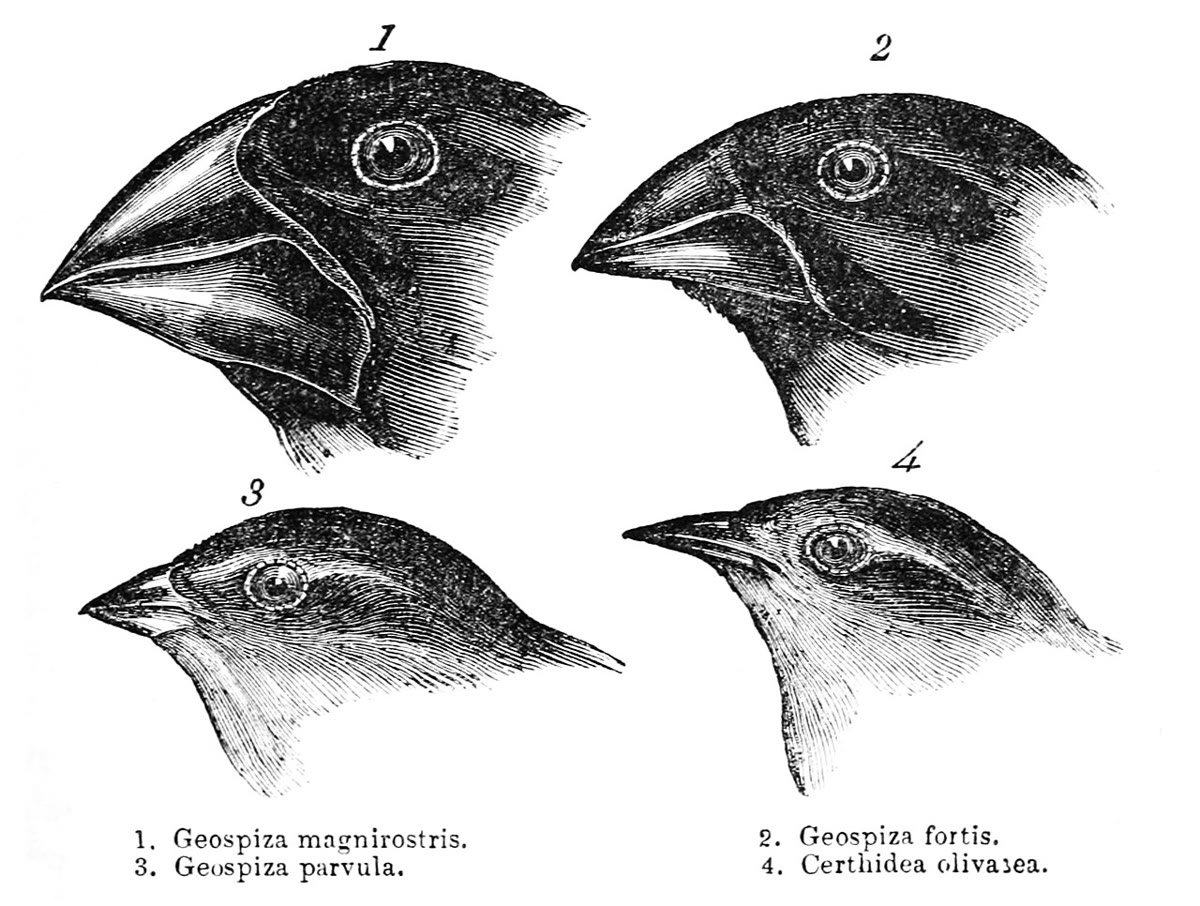
\includegraphics[width=0.44\linewidth]{images/book2/finches-gould.jpg}\hspace{0.04\linewidth}
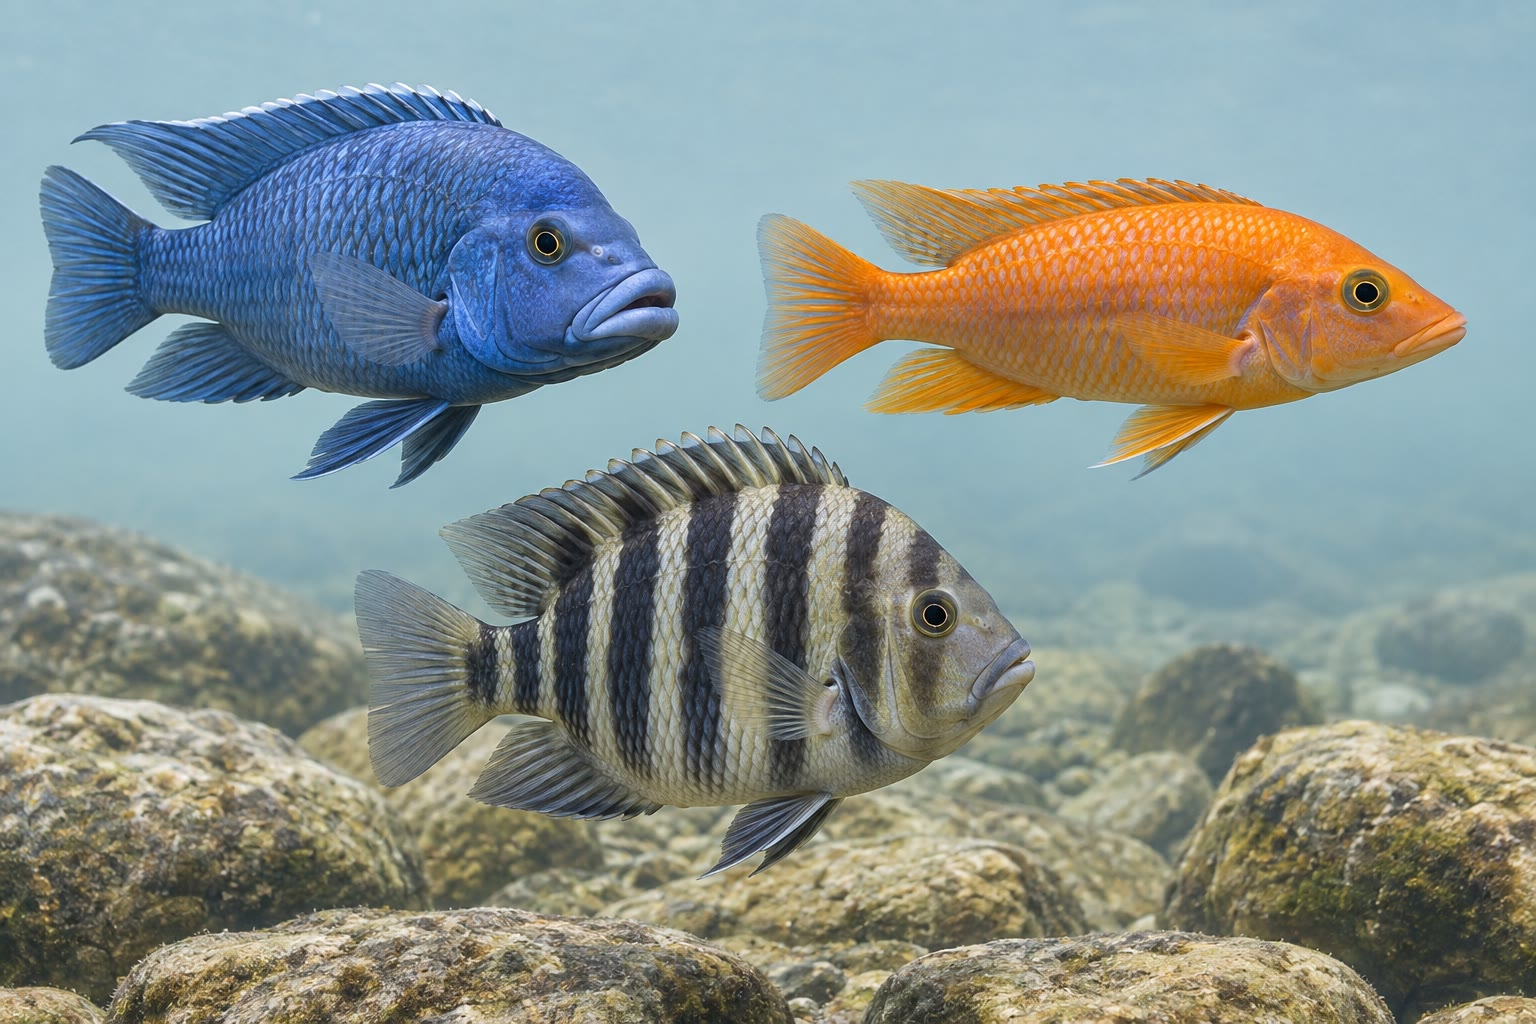
\includegraphics[width=0.44\linewidth]{images/book4/ai/b4-23-cichlids.jpg}

{\small Twee radiaties. Links: de vinken van Darwin zoals Gould ze in 1845
tekende, één kolonist die er vele werd, onderscheiden door hun snavels.
Rechts: cichliden van een Afrikaans meer, honderden soorten uit enkele
stichters, elk met een eigen bek en dieet.}
\end{omfigure}

\section{Macro-evolutie: het lange zicht}

\begin{proposition}[Tempo en wijze]\label{prop:b2:speciation:tempo}
\index{onderbroken evenwicht}\index{gradualisme}\index{massa-extinctie}
In enkele tientallen generaties veranderde de vlinder van kleur en de vink van
snavel; over miljoenen jaren toont het fossielenbestand lijnen die lange tijd
nauwelijks veranderen en dan, in een geologisch ogenblik van enkele duizenden
jaren, worden vervangen door een duidelijk verschillende afstammeling ---
\emph{\omterm{prop:b2:speciation:tempo}{onderbroken evenwicht}}, en zo ziet \omterm{prop:b2:speciation:modes}{allopatrische soortvorming} in kleine
perifere populaties, gevolgd door hun uitbreiding, eruit wanneer men om de
honderdduizend jaar een monster neemt; en het toont andere lijnen, waaronder
de paarden, die geleidelijk over tientallen soorten veranderen. Boven het
niveau van de soort is het bestand er een van vervanging: de meeste soorten
bestaan één tot tien miljoen jaar, de \emph{achtergrondextinctie} bedraagt
ongeveer één soort op een miljoen per jaar, en vijf keer --- aan het eind van
het Ordovicium, Devoon, Perm (toen negen tiende van de mariene soorten
verdween), Trias en Krijt --- verwijderde een \emph{massa-extinctie} binnen
enkele honderdduizenden jaren het meeste van wat er leefde en begon het spel
opnieuw, terwijl de overlevenden uitwaaierden in de vrijgekomen niches: de
zoogdieren in de wereld van de dinosauriërs na de planetoïde van 66 miljoen
jaar geleden. Macro-evolutie is het patroon dat de micro-evolutie van dit en
het vorige hoofdstuk heeft getekend, lang genoeg voortgezet en onderbroken door
catastrofes.
\end{proposition}

\begin{example}[Snelheden vergeleken]\label{ex:b2:speciation:rates}
Selectie op de vinken veranderde de snaveldiepte in één generatie met
\qty{4}{\%}; de hele radiatie van de Galápagos, veertien soorten uit één
stichter, duurde twee miljoen jaar; het verschil in lichaamsgrootte tussen een
muis en een olifant, zo'n $10^{5}$, zou door selectie met de sterkte van die
bij de vinken in enkele honderden generaties kunnen ontstaan --- en het
bestand laat zien dat het veertig miljoen jaar duurde. De paradox verdwijnt
wanneer men opmerkt dat selectie zelden lang in dezelfde richting duwt: ze
keert om met het weer, zoals op Daphne Major in het jaar na de droogte, en
\omterm{prop:b2:population-genetics:kinds}{stabiliserende selectie} houdt de meeste lijnen waar ze zijn. Aanhoudende
verandering is zeldzaam, en daarom is soortvorming, die ze nodig heeft, traag
--- en daarom gaan, wanneer de wereld snel verandert, zoals in
\cref{ch:b2:global-change}, de lijnen verloren die niet kunnen volgen.
\end{example}

\section{Opgaven}

\begin{exercise}[$\star$]\label{exo:b2:speciation:1}
Formuleer het biologische \omterm{def:b2:speciation:species}{soortbegrip} en geef drie gevallen waarin het niet
kan worden toegepast, met het begrip dat dan wordt gebruikt.
\end{exercise}

\begin{exercise}[$\star$]\label{exo:b2:speciation:2}
Deel in als prezygotisch of postzygotisch: twee kikkers die zich in
verschillende maanden voortplanten; een muilezel; een zaadcel van een zee-egel
die zich niet aan de eicel van een andere soort kan binden; hybride planten
die krachtig zijn maar waarvan de zaden niet kiemen; twee krekels met een
verschillende zang.
\end{exercise}

\begin{exercise}[$\star$]\label{exo:b2:speciation:3}
Definieer allopatrische, peripatrische, sympatrische en \omterm{prop:b2:speciation:modes}{parapatrische
soortvorming}, met van elk een voorbeeld.
\end{exercise}

\begin{exercise}[$\star$]\label{exo:b2:speciation:4}
Formuleer de vier uitkomsten van concurrentie volgens Lotka--Volterra en de
voorwaarde voor stabiele coëxistentie in woorden.
\end{exercise}

\begin{exercise}[$\star\star$]\label{exo:b2:speciation:5}
Bereken met $K_1 = 1000$, $K_2 = 800$, $\alpha = 0.5$, $\beta = 0.6$
de evenwichtsdichtheden en controleer dat elke soort de draagkracht van de
andere kan binnendringen.
\end{exercise}

\begin{exercise}[$\star\star$]\label{exo:b2:speciation:6}
Met $K_1 = 1000$, $K_2 = 800$, $\alpha = 1.5$, $\beta = 0.3$: welke
soort wint, en waarom? En als $\alpha = 1.5$ en $\beta = 1.5$?
\end{exercise}

\begin{exercise}[$\star\star$]\label{exo:b2:speciation:7}
In een diploïde populatie ontstaat een tetraploïde. Geef de chromosoomaantallen
van zijn gameten, van een kruising met de diploïde, en van de gameten van die
hybride, en leg uit waarom de tetraploïde meteen geïsoleerd is. Waarom
blijft hij toch meestal niet bestaan?
\end{exercise}

\begin{exercise}[$\star\star$]\label{exo:b2:speciation:8}
Twee populaties hebben sinds hun splitsing elk 10 substituties gefixeerd,
en elk paar nieuwe \omterm{def:b2:meiosis-heredity:vocabulary}{allelen} van de twee kanten is onverenigbaar
met kans $0.01$. Bereken het verwachte aantal
onverenigbaarheden nu, en na elk 30 substituties. Wat voorspelt dit over
het verband tussen isolatie en tijd?
\end{exercise}

\begin{exercise}[$\star\star$]\label{exo:b2:speciation:9}
Bereken de breedte van een \omterm{prop:b2:speciation:reinforcement}{hybridisatiezone} bij een verspreiding $\sigma =
\qty{2}{km}$ per generatie en een nadeel voor hybriden $s = 0.05$, en
bij $\sigma = \qty{0.3}{km}$ en $s = 0.4$. Welke zone zal eerder in
versterking eindigen, en waarom?
\end{exercise}

\begin{exercise}[$\star\star\star$]\label{exo:b2:speciation:10}
Twee vinkensoorten concurreren om zaden met $\alpha = \beta = 0.9$ en
$K_1 = K_2 = 500$. Leven ze samen? Kenmerkverschuiving verlaagt
$\alpha$ en $\beta$ tot $0.4$: bereken het evenwicht opnieuw. Leg met
de isoclinen uit wat de verschuiving heeft gedaan.
\end{exercise}

\begin{exercise}[$\star\star\star$]\label{exo:b2:speciation:11}
De Grants stelden vast dat na de droogte van 2004 de gemiddelde snaveldiepte
van de middelste grondvink met \qty{0.7}{mm} daalde bij $h^{2} = 0.7$,
terwijl de overlevenden een snavel hadden die \qty{1}{mm} kleiner was dan die
van de populatie. Controleer de respons met de \omterm{thm:b2:population-genetics:heritability}{fokkersvergelijking}, en
leg uit waarom de aanwezigheid van de grote grondvink, en niet de droogte
alleen, de richting van de verandering bepaalde.
\end{exercise}

\begin{exercise}[$\star\star\star$]\label{exo:b2:speciation:12}
``Soorten ontstaan bij toeval en worden door selectie in stand gehouden.''
Bespreek dit met het model met twee loci, versterking en de rol van de geografie.
\end{exercise}

\section{Vraagstuk: twee vinken op een eiland}

\begin{problem}[{Weekendvraagstuk --- een inheemse vink ontmoet een
indringer: hun concurrentie geanalyseerd in het fasevlak, de verschuiving van
de snavel van de inheemse soort voorspeld met de fokkersvergelijking, en de
isolatie tussen hen afgemeten aan een hybridisatiezone, met als besluit de
evenwichtsdichtheden, de verschuiving van de snavel en de breedte van de
cline}]
\label{pb:b2:speciation:1}
Inheemse soort 1: $K_1 = 1200$, $r_1 = 0.5$ per jaar; indringende
soort 2: $K_2 = 400$. Vóór de verschuiving $\alpha = 0.9$, $\beta =
0.3$; een droogte halveert één jaar lang beide draagkrachten. Snaveldiepte
van soort 1: gemiddeld \qty{9.5}{mm}, standaardafwijking
\qty{0.8}{mm}, $h^{2} = 0.7$. Parameters van de \omterm{prop:b2:speciation:reinforcement}{hybridisatiezone}: $\sigma =
\qty{0.5}{km}$, $s = 0.2$.

\medskip
\noindent\textbf{Deel I --- De invasie.}
\begin{enumerate}
  \item Schrijf de twee isoclinen en hun snijpunten met de assen op.
  \item Kan soort 2 soort 1 op $K_1$ binnendringen? Kan soort 1
        soort 2 op $K_2$ binnendringen? Trek een conclusie over de uitkomst.
  \item Bereken de evenwichtsdichtheden.
  \item Bereken $\mathrm{d}N_1/\mathrm{d}t$ op het moment dat soort 2
        aankomt met $N_2 = 20$ en $N_1 = 1200$. Wat betekent het
        teken?
  \item Tijdens de droogte worden beide $K$ gehalveerd. Bereken het
        evenwicht opnieuw en zeg wat er met de aantallen van elke soort gebeurt.
  \item Waarom is het effect van de indringer op de inheemse soort ($\alpha = 0.9$)
        groter dan dat van de inheemse soort op de indringer ($\beta = 0.3$)?
\end{enumerate}

\medskip
\noindent\textbf{Deel II --- Verschuiving.}
Tijdens de droogte concurreren de inheemse individuen met de grootste snavels
het meest met de indringer en sterven ze: de overlevenden hebben een
gemiddelde snavel van \qty{9.0}{mm}.
\begin{enumerate}[resume]
  \item Bereken het selectiedifferentieel en de respons.
  \item Geef de gemiddelde snavel van de volgende generatie.
  \item Na de verschuiving daalt $\alpha$ tot $0.5$. Bereken het
        evenwicht opnieuw (met de oorspronkelijke $K$).
  \item Leg uit wat de verschuiving met de isocline van soort 1 deed.
  \item Als selectie met deze sterkte elk jaar werkte, hoeveel
        jaar zou het dan duren om de snavel \qty{2}{mm} te verschuiven? Waarom
        gebeurt dat niet?
  \item Vergelijk met de ouderdom van twee miljoen jaar van de radiatie en
        geef commentaar.
\end{enumerate}

\medskip
\noindent\textbf{Deel III --- Isolatie.}
De twee soorten kunnen hybridiseren; hybriden hebben tussenliggende snavels en
\omterm{def:b2:population-genetics:fitness}{fitness} $1 - s$.
\begin{enumerate}[resume]
  \item Noem de prezygotische barrière die hybridisatie bij de vinken van
        Darwin zeldzaam houdt, en één postzygotische kostenpost van de
        hybriden.
  \item Bereken de breedte van een \omterm{prop:b2:speciation:reinforcement}{hybridisatiezone} tussen hen voor $\sigma
        = \qty{0.5}{km}$, $s = 0.2$.
  \item Het eiland is \qty{1}{km} breed. Wat houdt dat in?
  \item Leg uit hoe versterking zou verlopen, en op welk kenmerk
        ze zou inwerken.
  \item Twee populaties van de inheemse soort op verschillende eilanden hebben
        sinds hun scheiding elk 15 substituties gefixeerd; paren zijn
        onverenigbaar met kans $0.005$. Bereken het verwachte aantal
        onverenigbaarheden en zeg of het soorten zijn.
  \item Zouden het biologische, het morfologische en het fylogenetische
        \omterm{def:b2:speciation:species}{soortbegrip} het over de twee eilandpopulaties eens zijn? Leg uit.
\end{enumerate}

\medskip
\noindent\textbf{Deel IV --- Het lange zicht.}
\begin{enumerate}[resume]
  \item Als een soort gemiddeld 5 miljoen jaar bestaat, wat is dan de
        achtergrondextinctie per soort per jaar? Hoeveel uitstervingen per
        jaar geeft dat voor een biota van 10 miljoen soorten?
  \item De huidige extinctiesnelheid wordt geschat op 100 tot 1000
        keer de achtergrond. Hoeveel soorten per jaar is dat?
  \item Een massa-extinctie verwijdert \qty{75}{\%} van de soorten in
        \num{100000} jaar. Vergelijk haar snelheid met de huidige.
  \item Leg in één zin uit waarom de overlevenden van een
        massa-extinctie uitwaaieren.
  \item Een lijn in het fossielenbestand verandert 3 miljoen jaar weinig
        en wordt dan binnen \num{20000} jaar vervangen door een duidelijk
        verschillende afstammeling. Benoem het patroon en geef de wijze van
        soortvorming die het voortbrengt.
  \item Hoeveel generaties aanhoudende selectie zouden, met de
        \qty{4}{\%} per generatie van de vink, de snaveldiepte verdubbelen?
        Waarom toont het fossielenbestand dat zulke veranderingen miljoenen
        jaren duren?
  \item Formuleer het resultaat: de uitkomst en het evenwicht van de
        concurrentie vóór en na de verschuiving, de verschuiving van de snavel
        in één generatie, en de breedte van de \omterm{prop:b2:speciation:reinforcement}{hybridisatiezone}.
\end{enumerate}
\end{problem}
